%%%%%%%%%%%%%%%%%%%%%%%%%%%%%%%%%%%%%%%%%%%%%%%%%%%%%%%%%%%%%%%%%%%%%%%%%%%%%%%%%%
\begin{frame}[fragile]\frametitle{}
\begin{center}
{\Large Sets}
\end{center}
\end{frame}

%%%%%%%%%%%%%%%%%%%%%%%%%%%%%%%%%%%%%%%%%%%%%%%%%%%%%%%%%%
\begin{frame}{Sets}
\begin{example}
The set consisting of all positive integers less than $10$ can be denoted by $\{1,2,3,4,5,6,7,8,9\}$.  $\{1,2,3,\ldots,9\}$ is also used since the general pattern is obvious.
\end{example}
\end{frame}


%%%%%%%%%%%%%%%%%%%%%%%%%%%%%%%%%%%%%%%%%%%%%%%%%%%%%%%%%%
\begin{frame}{Sets}
\begin{example}
Members of a set need not be numeric.  The set of all possible outcomes when tossing a coin is  $\{H,T\}$.
\end{example}
\end{frame}

%%%%%%%%%%%%%%%%%%%%%%%%%%%%%%%%%%%%%%%%%%%%%%%%%%%%%%%%%%
\begin{frame}{Set Builder Notation}
For example, $O=\{1,3,5,7,9\}$ can also be written as $$O=\{x: x \text{ is a positive odd integer less than } 10\}.$$

\begin{example} 
\begin{itemize}
\item $A=\{x: x \text{ is a positive even number less than }15\}=\{2,4,6,8,10,12,14\}$.
\item $B=\{n: n \text{ is a positive integer}\}=\{1,2,3,4,5,\ldots\}$.
\item $C=\{2n: n \text{ is a whole number and }1\leq n\leq 4\}=\{2,4,6,8\}$.
\end{itemize}
\end{example}
\end{frame}

%%%%%%%%%%%%%%%%%%%%%%%%%%%%%%%%%%%%%%%%%%%%%%%%%%%%%%%%%%
\begin{frame}{Some Basic Notations}

\begin{itemize}
\item $\emptyset$, The \underline{empty set}\index{empty set} (a set with \textit{no} elements). $\{\quad\}$ is also used. 
\item $\mathbb{N}=\{1,2,3,\ldots\}$, the set of natural numbers.\index{natural number}\index{$\mathbb{N}$}
\item $\mathbb{Z}=\{\ldots,-2,-1,0,1,2,\ldots\}$, the set of integers. \index{integer}\index{$\mathbb{Z}$}
\item $\mathbb{R}$ or $(-\infty,\infty)$, the set of real numbers. \index{real number}\index{$\mathbb{R}$}
\item $[a,b]$, the set of all real numbers $x$ such that $a\leq x \leq b$.
\item $(a,b)$, the set of all real numbers $x$ such that $a< x < b$. 
\item $(a,b]$, the set of all real numbers $x$ such that $a< x \leq  b$. 
\item $[a,b)$, the set of all real numbers $x$ such that $a\leq x< b$. 
\end{itemize}

\end{frame}

%%%%%%%%%%%%%%%%%%%%%%%%%%%%%%%%%%%%%%%%%%%%%%%%%%%%%%%%%%
\begin{frame}{Subsets and Equality}
\begin{definition} A set $A$ is said to be a \underline{subset} of another set $B$  if every element of $A$ is also an element of $B$.  We use the notation $A\subseteq B$.  Two sets $A$ and $B$ are said to be \underline{equal} (notation $A=B$)  if they have the same elements.  In other words, $A$ and $B$ are equal if $A\subseteq B$ and $B\subseteq A$.
\end{definition}
\end{frame}

%%%%%%%%%%%%%%%%%%%%%%%%%%%%%%%%%%%%%%%%%%%%%%%%%%%%%%%%%%
\begin{frame}{Subsets and Equality}
\begin{example} $\{2,3,5\}\subseteq \{-1,2,3,5,7\}$.  However, $\{1,2,3,4\} \nsubseteq \{1,3,4,5,6,7\}$,  because $2\notin \{1,3,4,5,6,7\}$.
\end{example}

\begin{example} By definition, $\mathbb{N}\subseteq \mathbb{Z}\subseteq \mathbb{R}$.
\end{example}
\end{frame}

%%%%%%%%%%%%%%%%%%%%%%%%%%%%%%%%%%%%%%%%%%%%%%%%%%%%%%%%%%
\begin{frame}{Set Operations}
 Let $A$ and $B$ be sets. 
\begin{itemize}
\item The \underline{union} of $A$ and $B$, denoted by $A\cup B$, is the set that contains those elements that are either in $A$ or $B$, or in both.  In other words, $A\cup B=\{x: x\in A \text{ or } x\in B\}$. 
\item The \underline{intersection} of $A$ and $B$, denoted by $A\cap B$, is the set that contains those elements in both $A$ and $B$.  In other words, $A\cap B=\{x: x\in A \text{ and } x\in B\}$. 
\item Two sets are said to be \underline{disjoint} if their intersection is the empty set. 
\item Let $S$ be the universal set (the set of all elements under consideration. It depends on the context).  Then the \underline{complement} $A^c$ of $A$ is defined to be the set of all elements in $S$ that are not in $A$.
\end{itemize}

\end{frame}

%%%%%%%%%%%%%%%%%%%%%%%%%%%%%%%%%%%%%%%%%%%%%%%%%%%%%%%%%%
\begin{frame}{Set Operations, continued}
\begin{example} Let $A=\{1,3,4,5\}$ and $B=\{1,2,3\}$, then $A\cup B=\{1,2,3,4,5\}$ and $A\cap B=\{1,3\}$.
\end{example}

\begin{center}
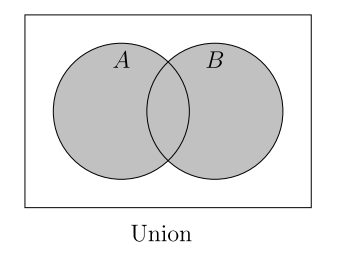
\includegraphics[width=0.4\linewidth,keepaspectratio]{setun}
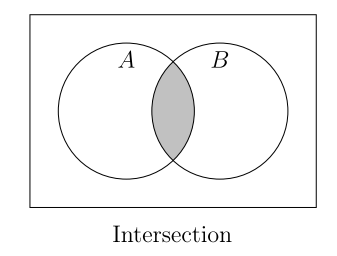
\includegraphics[width=0.4\linewidth,keepaspectratio]{setint}
\end{center}
\end{frame}

%%%%%%%%%%%%%%%%%%%%%%%%%%%%%%%%%%%%%%%%%%%%%%%%%%%%%%%%%%
\begin{frame}{Set Operations, continued}
\begin{example}
If $P=(-\infty, 2)$ and $Q=[-1,\infty)$, then $P\cap Q=[-1,2)$ and $P\cup Q=(-\infty,\infty)=\mathbb{R}$.
\end{example}
\end{frame}

%%%%%%%%%%%%%%%%%%%%%%%%%%%%%%%%%%%%%%%%%%%%%%%%%%%%%%%%%%
\begin{frame}{Set Operations, continued}
\begin{example} Let $O=\{2k+1: k\in \mathbb{Z}\}$ and $E=\{2k: k\in \mathbb{Z}\}$, then $O$ and $E$ are disjoint.  If one takes $\mathbb{Z}$ as the universal set, then $O^c=E$ and $E^c=O$.
\end{example}

\end{frame}


%%%%%%%%%%%%%%%%%%%%%%%%%%%%%%%%%%%%%%%%%%%%%%%%%%%%%%%%%%
\begin{frame}{Cardinality of the Union of Sets}
Let $|S|$ denote the number of elements of a set $S$.  Obviously, $A\cup B$ contains both $A$ and $B$, so $|A\cup B|\geq |A|$ and $|A\cup B|\geq |B|$.  But exactly how many elements are there in $A\cup B$?

\begin{theorem} Let $A,B$ be sets with finitely many elements, then
$$|A\cup B|=|A|+|B|-|A\cap B|.$$  In particular, if $A$ and $B$ are disjoint, then $|A\cup B|=|A|+|B|$.
\end{theorem}

\end{frame}


%%%%%%%%%%%%%%%%%%%%%%%%%%%%%%%%%%%%%%%%%%%%%%%%%%%%%%%%%%
\begin{frame}{Cardinality of the Union of Sets}

\begin{theorem} Let $A,B,C$ be sets with finitely many elements, then
$$|A\cup B \cup C|=|A|+|B|+|C|-|A\cap B|-|B\cap C|-|A\cap C|+|A\cap B \cap C|.$$ 
\end{theorem}
\end{frame}

